\documentclass[../main.tex]{subfiles}
%!TEX root = ./appendixDragAnalysis.tex
\graphicspath {{../}}

\begin{document}
\subsection{Previous Drag Analysis}

Before knowing that the airship envelope needed to be parametrizable, drag values were initially computed using SolidWorks, by its built in Flow Simulation add-on. Simulations were conducted from 2m/s to 20m/s, at intervals of 2m/s. Skin Friction Drag and Regular Drag were computed and summed to obtain total drag for each speed. A table with the results from the simulations can be seen in Table \ref{tbl:DracTable}.

\begin{table}[H]
	\centering
	\caption{Raw Data From SolidWorks Flow Simulation}
	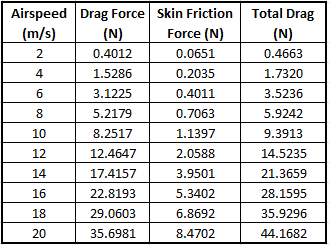
\includegraphics[width=.5\linewidth]{img/drag/dragTable.PNG}
	\label{tbl:DracTable}
\end{table}

\begin{figure}[H]
	\centering
	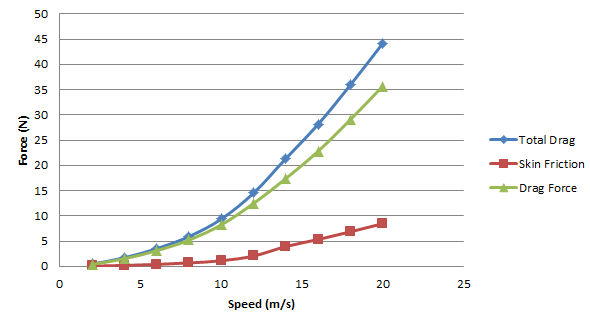
\includegraphics[width=\linewidth]{img/drag/dragForces.PNG}
	\caption{Drag Force Curves Computed From SolidWorks Flow Simulation}
	\label{fig:dragForces}
\end{figure}

The values of simulated drag were then sent into MATLAB and a curve fitting analysis was completed. A graph of the raw data versus the fitted curve is shown in Figure \ref{fig:dragForces}.

\begin{figure}[H]
	\centering
	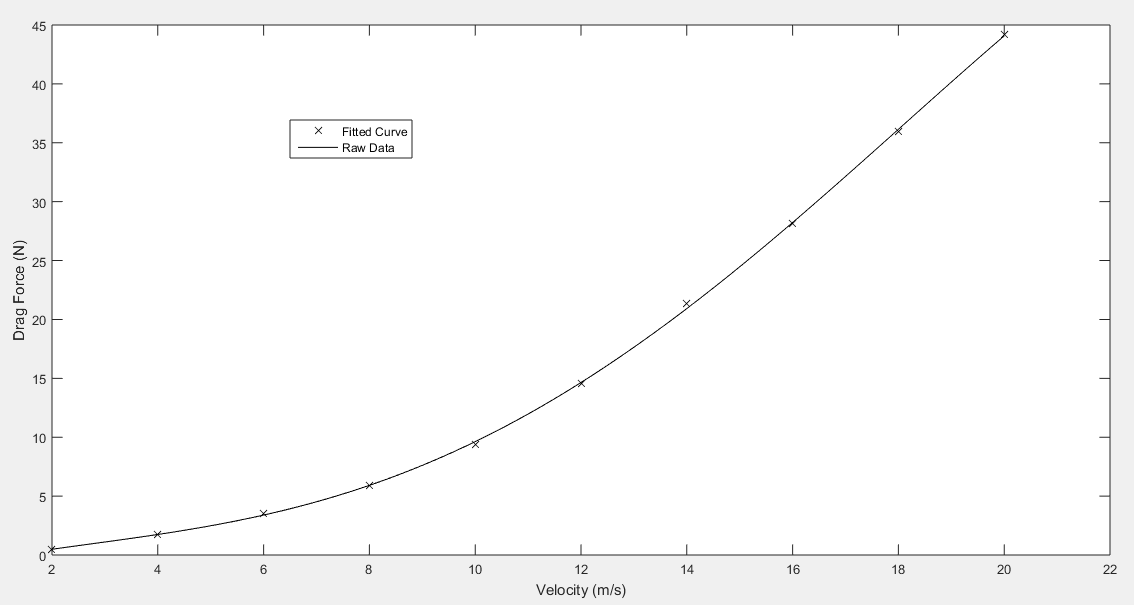
\includegraphics[width=\linewidth]{img/drag/curveFit.PNG}
	\caption{Drag Force Curves Computed From SolidWorks Flow Simulation}
	\label{fig:curveFit}
\end{figure}

The equation from the curve (generated from MATLAB) was found to be:

\begin{equation} \label{dragEqn}
	D(v) = -0.0003545v^4 + 0.014182v^3 -0.05385v^2 + 0.45054v -0.087259
\end{equation}

Where $ D $ is the drag force and $ v $ is the airship speed, in $m/s$. Equation \ref{dragEqn} is what is used throughout the report to obtain drag forces.\\

\end{document}